\section{Task 3 --- Graph Embedding over Homogeneous Structures}
\label{p1:sec:main}

\subsection{Approach}
\label{p1:sec:approach}

All four notebook TODOs are implemented.  Every provided helper --- data loading, the
cached adjacency lookups, the whole evaluation toolset of section~5 and
\texttt{run\_experiment} --- is used verbatim, with \texttt{RANDOM\_SEED}${}=0$.
Loading reproduces the published statistics exactly:
$7{,}624$ users, $19{,}464$ observed edges, $666$ isolated users, mean degree $5.106$,
max degree $153$, $734$ components, and $4{,}171\times 21$ validation/test queries.

\paragraph{\texttt{sample\_walks}.}
A strategy is nothing but a transition rule; the \emph{walk budget is identical for every
strategy} ($10$ walks of length $40$ from each of the $6{,}958$ non-isolated users, giving
$69{,}580$ walks in every run).  The $666$ isolated users return \texttt{[]}, as the
docstring permits, and therefore keep a zero embedding row.  Five transition rules are
compared, giving the seven configurations of Table~\ref{p1:tab:comparison} (node2vec is
run at three $(p,q)$ settings):

\begin{center}\small
\begin{tabular}{@{}llp{6.6cm}@{}}
\toprule
strategy & transition rule $P(x \mid \cdot)$ & hypothesis being tested \\
\midrule
DeepWalk & uniform over $N(v)$ & baseline: unbiased 1st-order walk \\
node2vec & $\propto 1/p,\,1,\,1/q$ by distance to $t$ & $q<1$ outward (homophily), $q>1$ inward (structural equivalence) \\
RWR & uniform, teleport to \texttt{start} w.p.\ $r$ & a strongly \emph{personalised} context should sharpen pairwise proximity, at the cost of global community signal \\
deg-corrected & $\propto \deg(x)^{-\alpha}$ & uniform walks over-visit hubs; equalising visit counts should lift the low-degree source buckets \\
triadic & $\propto 1 + |N(v)\cap N(x)|$ & preferring triangle-closing steps keeps the walk inside a community, i.e.\ maximal homophily \\
\bottomrule
\end{tabular}
\end{center}

\noindent
RWR, deg-corrected and triadic are my own additions.  node2vec uses the standard
$O(1)$ rejection sampler rather than materialising alias tables, which keeps a
second-order walk at $1.3\,$s for the whole corpus.

\paragraph{\texttt{train\_embedding}.}
Skip-Gram with negative sampling (\texttt{gensim.Word2Vec}, \texttt{sg=1}) over the walk
corpus.  I set \texttt{sample=0}, i.e.\ \emph{no} frequent-token subsampling: subsampling
would itself down-weight hubs and so half-implement the deg-corrected strategy,
confounding that comparison.  \texttt{workers=1} makes every run bit-exactly reproducible
(gensim's multi-threaded training is not deterministic).

\paragraph{Downstream models (held fixed).}
As the notebook demands, the link predictor and the country classifier are the very same
code for every row of the comparison table; the embedding is the only thing that changes.  Both $\ell_2$-normalise $Z$ row-wise (zero rows stay zero), standardise, and fit
a logistic regression.  A pair $(u,v)$ becomes
\[
  \phi(u,v)=\bigl[\,\underbrace{z_u \odot z_v}_{\text{Hadamard}},\;
                   \underbrace{|z_u-z_v|}_{\text{abs.\ diff.}},\;
                   \cos(z_u,z_v),\; z_u^\top z_v,\; \|z_u-z_v\|_2 \,\bigr]
  \in \mathbb{R}^{2d+3},
\]
the node2vec paper's two best binary operators concatenated with three scalar similarities.
\texttt{score} returns the continuous \texttt{decision\_function}, so higher always means
"more likely an edge".

\begin{table}[H]
\centering\small
\caption*{Fixed hyper-parameters (identical in every run).}
\begin{tabular}{@{}ll@{\hspace{2em}}ll@{}}
\toprule
walks per node & $10$                  & embedding dim.\ $d$ & $128$ \\
walk length    & $40$                  & Skip-Gram window    & $5$ \\
corpus size    & $69{,}580$ walks      & negative samples    & $5$ \\
seed           & $0$ (also $1,2$)      & epochs              & $5$ \\
LP regulariser & $C\!\in\!\{0.1,1,10\}$, chosen by val.\ MRR & subsampling & off (\texttt{sample=0}) \\
CC regulariser & $C\!\in\!\{0.1,1,10,100\}$, chosen by val.\ micro-F1 & solver & lbfgs \\
\bottomrule
\end{tabular}
\end{table}

\subsection{Implementation}
\label{p1:sec:code}

Only the code I wrote is listed; the provided scaffolding is omitted.

\lstdefinestyle{p1code}{basicstyle=\ttfamily\scriptsize,breaklines=true,language=Python,
        keywordstyle=\color{blue!60!black},commentstyle=\color{green!35!black},
        stringstyle=\color{red!50!black},showstringspaces=false,columns=fullflexible,
        captionpos=b}

\begin{lstlisting}[style=p1code,caption={TODO 1 --- \texttt{sample\_walks}}]
def sample_walks(self, G, start):
    """`num_walks` walks of length `walk_length`, all beginning at `start`."""
    adj, deg = adjacency_lookups(G)
    if deg[start] == 0:                    # isolated node -> no walks (allowed)
        return []
    rng, L, R, strat = self._rng, self.walk_length, self.num_walks, self.strategy

    if strat == "node2vec":                # 2nd-order, O(1) rejection sampling
        NBR = self._nbr_lists(G)           # cached sorted neighbour lists
        p, q = self.params["p"], self.params["q"]
        inv_p, inv_q, wmax = 1/p, 1/q, max(1/p, 1.0, 1/q)
        walks = []
        for _ in range(R):
            walk = [start, rng.choice(NBR[start])]      # 1st step unbiased
            while len(walk) < L:
                cur, prev = walk[-1], walk[-2]
                cn, prev_nbrs = NBR[cur], adj[prev]
                while True:
                    x = rng.choice(cn)
                    w = inv_p if x == prev else (1.0 if x in prev_nbrs else inv_q)
                    if rng.random() * wmax < w:
                        break
                walk.append(x)
            walks.append(walk)
        return walks

    if strat in ("degcorr", "triadic"):    # 1st-order, edge-weighted
        tables = self._weighted_tables(G)  # per node: (nbrs, cumulative weights)
        walks = []                         # degcorr: w(x) = deg(x)**-alpha
        for _ in range(R):                 # triadic: w(x) = 1 + |N(cur) & N(x)|
            walk = [start]
            while len(walk) < L:
                nbrs, cum = tables[walk[-1]]
                walk.append(rng.choices(nbrs, cum_weights=cum, k=1)[0])
            walks.append(walk)
        return walks

    NBR = self._nbr_lists(G)               # "uniform" (DeepWalk) and "rwr"
    restart = self.params.get("restart", 0.0) if strat == "rwr" else 0.0
    walks = []
    for _ in range(R):
        walk = [start]
        while len(walk) < L:
            if restart and rng.random() < restart:
                walk.append(start)         # teleport home, then carry on
            else:
                walk.append(rng.choice(NBR[walk[-1]]))
        walks.append(walk)
    return walks
\end{lstlisting}

\begin{lstlisting}[style=p1code,caption={TODO 2 --- \texttt{train\_embedding}}]
def train_embedding(self, walks, n_nodes):
    d = self.params.get("dim", 128)
    model = Word2Vec(sentences=[[str(v) for v in w] for w in walks],
                     vector_size=d, window=self.params.get("window", 5),
                     sg=1, hs=0, negative=self.params.get("negative", 5),
                     epochs=self.params.get("epochs", 5),
                     min_count=0, sample=0, seed=self.seed, workers=1)
    Z = np.zeros((n_nodes, d), dtype=float)   # nodes never walked keep a zero row
    Z[[int(k) for k in model.wv.index_to_key]] = model.wv.vectors
    return Z
\end{lstlisting}

\begin{lstlisting}[style=p1code,caption={TODO 3a --- \texttt{LinkPredictor} (and the pair feature map)}]
def _unit(Z):                       # row-wise L2 norm; all-zero rows stay zero
    n = np.linalg.norm(Z, axis=1, keepdims=True)
    return Z / np.where(n == 0.0, 1.0, n)

def _pair_features(Z, pairs):       # (n_q, n_cand, 2) -> (n_q*n_cand, 2d+3)
    u, v = Z[pairs[..., 0]].reshape(-1, Z.shape[1]), Z[pairs[..., 1]].reshape(-1, Z.shape[1])
    had, dif = u * v, np.abs(u - v)
    dot = had.sum(1, keepdims=True)
    l2  = np.linalg.norm(u - v, axis=1, keepdims=True)
    cos = dot / np.maximum(np.linalg.norm(u, axis=1, keepdims=True)
                           * np.linalg.norm(v, axis=1, keepdims=True), 1e-12)
    return np.hstack([had, dif, cos, dot, l2])

class LinkPredictor:
    C_GRID = (0.1, 1.0, 10.0)

    def fit(self, Z, pairs_train, y_train, pairs_val, y_val):
        Zn  = _unit(np.asarray(Z, dtype=float))
        Xtr = _pair_features(Zn, pairs_train)
        self.scaler = StandardScaler().fit(Xtr)
        Xtr, ytr = self.scaler.transform(Xtr), np.asarray(y_train).ravel()
        Xva = self.scaler.transform(_pair_features(Zn, pairs_val))
        nq, nc  = pairs_val.shape[:2]
        pos_val = np.argmax(np.asarray(y_val), axis=1)

        best = (-1.0, None, None)
        for C in self.C_GRID:                    # model selection on validation MRR
            clf = LogisticRegression(C=C, max_iter=2000, random_state=RANDOM_SEED)
            clf.fit(Xtr, ytr)
            s    = clf.decision_function(Xva).reshape(nq, nc)
            rank = 1 + (s > s[np.arange(nq), pos_val][:, None]).sum(1)
            mrr  = float(np.mean(1.0 / rank))
            if mrr > best[0]:
                best = (mrr, clf, C)
        self.val_mrr_, self.clf, self.C_ = best
        return self

    def score(self, Z, pairs):                   # continuous, higher = more likely
        X = self.scaler.transform(_pair_features(_unit(np.asarray(Z, float)), pairs))
        return self.clf.decision_function(X).reshape(pairs.shape[:2])
\end{lstlisting}

\begin{lstlisting}[style=p1code,caption={TODO 3b --- \texttt{CountryClassifier}}]
class CountryClassifier:
    C_GRID = (0.1, 1.0, 10.0, 100.0)

    def fit(self, Z_train, y_train, Z_val, y_val):
        Xtr = _unit(np.asarray(Z_train, dtype=float))
        self.scaler = StandardScaler().fit(Xtr)
        Xtr = self.scaler.transform(Xtr)
        Xva = self.scaler.transform(_unit(np.asarray(Z_val, dtype=float)))
        best = (-1.0, None, None)
        for C in self.C_GRID:                    # selection on validation micro-F1
            clf = LogisticRegression(C=C, max_iter=5000, random_state=RANDOM_SEED)
            clf.fit(Xtr, y_train)
            acc = float((clf.predict(Xva) == np.asarray(y_val)).mean())
            if acc > best[0]:
                best = (acc, clf, C)
        self.val_micro_f1_, self.clf, self.C_ = best
        return self

    def predict(self, Z):
        return self.clf.predict(self.scaler.transform(_unit(np.asarray(Z, float))))
\end{lstlisting}

\subsection{Results}
\label{p1:sec:results}

Every number below was measured on this machine.  Because the seven strategies turned out
to lie close together, I ran the \emph{whole} protocol three times (seeds $0,1,2$; the
seed drives both the walk sampling and the Skip-Gram initialisation) and report the mean,
so that a difference can be compared against the run-to-run noise.  Table~\ref{p1:tab:comparison}
is \texttt{comparison\_table()} averaged over those three runs, with one added column
(validation macro-F1, which \texttt{run\_experiment} does not itself record).

\begin{table}[H]
\centering\footnotesize
\caption{The scalar metrics of \texttt{comparison\_table()} together with a validation
macro-F1 column that \texttt{run\_experiment} does not record, mean over seeds
$\{0,1,2\}$; its six \texttt{val\_hit@1\_deg*} columns are given in full in
Table~\ref{p1:tab:valdeg}.  Best per column in bold.  The last two rows give the mean
within-strategy standard deviation over the three seeds --- the noise floor a difference
must beat --- and the best-minus-worst spread expressed in those units.  Columns marked
$\dagger$ are measured on the split that \texttt{fit} selects $C$ on and are therefore
optimistic; the test columns are the ones that carry the argument.}
\label{p1:tab:comparison}
\setlength{\tabcolsep}{3.2pt}
\begin{tabular}{@{}lcccccccc@{}}
\toprule
& \multicolumn{4}{c}{friend recommendation} & \multicolumn{4}{c}{country classification} \\
\cmidrule(lr){2-5}\cmidrule(lr){6-9}
strategy & val H@1$^\dagger$ & val MRR$^\dagger$ & test H@1 & test MRR & val mi-F1$^\dagger$ & val ma-F1 & test mi-F1 & test ma-F1 \\
\midrule
DeepWalk & 0.6040 & 0.7227 & 0.6009 & 0.7207 & 0.7641 & 0.6639 & 0.7629 & 0.6833 \\
n2v $p{=}1,q{=}0.5$ & 0.5995 & 0.7202 & 0.5959 & 0.7184 & 0.7636 & 0.6621 & 0.7621 & 0.6825 \\
n2v $p{=}1,q{=}2$ & 0.6027 & 0.7210 & 0.6011 & 0.7196 & 0.7619 & 0.6467 & 0.7607 & 0.6802 \\
n2v $p{=}q{=}0.25$ & 0.6039 & 0.7217 & 0.6061 & 0.7228 & 0.7610 & 0.6581 & 0.7628 & 0.6796 \\
RWR $r{=}0.15$ & 0.5870 & 0.7119 & 0.5889 & 0.7124 & 0.7637 & 0.6521 & 0.7620 & 0.6733 \\
deg-corr.\ $\alpha{=}1$ & 0.6003 & 0.7144 & 0.5990 & 0.7121 & 0.7575 & 0.6421 & 0.7607 & 0.6781 \\
triadic & \textbf{0.6066} & \textbf{0.7247} & \textbf{0.6087} & \textbf{0.7248} & \textbf{0.7645} & \textbf{0.6833} & \textbf{0.7661} & \textbf{0.6974} \\
\midrule
\textit{noise floor} & 0.0028 & 0.0021 & 0.0048 & 0.0031 & 0.0055 & 0.0077 & 0.0032 & 0.0062 \\
\textit{spread} / noise & $7.0\times$ & $6.0\times$ & $4.1\times$ & $4.2\times$ & $1.3\times$ & $5.4\times$ & $1.7\times$ & $3.9\times$ \\
\bottomrule
\end{tabular}
\end{table}

\begin{figure}[H]
\centering
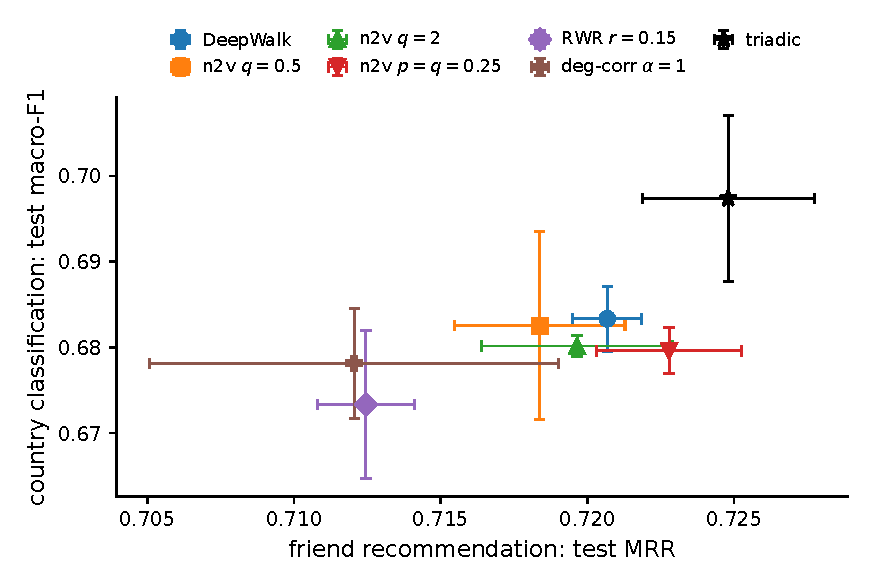
\includegraphics[width=0.78\textwidth]{fig_p1_tradeoff.pdf}
\caption{Each strategy on both tasks at once; error bars are $\pm 1$ sd over the three
seeds.  There is no trade-off frontier --- the triadic walk sits alone in the top-right
corner.}
\label{p1:fig:tradeoff}
\end{figure}

\paragraph{Per-source-degree breakdown.}
Table~\ref{p1:tab:degree} gives \texttt{breakdown\_by\_source\_degree} on the test split for
the baseline, the best strategy and the worst, with both metrics;
Figure~\ref{p1:fig:degree} plots the Hit@1 half of it with seed error bars.
Table~\ref{p1:tab:valdeg} then gives the validation Hit@1 breakdown for \emph{all seven}
strategies --- these are literally the six \texttt{val\_hit@1\_deg*} columns that
\texttt{run\_experiment} records, which is why they are on the validation split.
Note that triadic, which wins every aggregate column of Table~\ref{p1:tab:comparison},
wins only three of the six degree buckets there: \mbox{node2vec} $p{=}q{=}0.25$ takes the
cold and $8$--$15$ buckets and $q{=}2$ ties the $2$--$3$ bucket.  Per-bucket margins are
small and the buckets are $3$--$20\times$ smaller than the full split, so individual cells
are much noisier than the aggregates; the consistent pattern is the one visible in the two
highest-degree buckets, not any single cell.

\begin{table}[H]
\centering\small
\caption{\texttt{breakdown\_by\_source\_degree}, test split, mean over seeds $\{0,1,2\}$,
by number of friends the \emph{source} user has in $G_{\mathrm{train}}$: the baseline, the
best strategy and the worst.}
\label{p1:tab:degree}
\begin{tabular}{@{}lccccccc@{}}
\toprule
 & & \multicolumn{2}{c}{DeepWalk (baseline)} & \multicolumn{2}{c}{triadic (best)} & \multicolumn{2}{c}{RWR (worst)} \\
\cmidrule(lr){3-4}\cmidrule(lr){5-6}\cmidrule(lr){7-8}
source degree & $n$ & Hit@1 & MRR & Hit@1 & MRR & Hit@1 & MRR \\
\midrule
$0$ (cold) & 216 & 0.0447 & 0.1887 & 0.0293 & 0.1759 & 0.0447 & 0.1825 \\
$1$ & 266 & 0.4386 & 0.5672 & 0.4423 & 0.5680 & \textbf{0.4499} & \textbf{0.5705} \\
$2$--$3$ & 469 & 0.5615 & 0.6823 & \textbf{0.5672} & \textbf{0.6852} & 0.5529 & 0.6752 \\
$4$--$7$ & 842 & 0.6675 & 0.7709 & \textbf{0.6710} & \textbf{0.7732} & 0.6524 & 0.7616 \\
$8$--$15$ & 939 & 0.6784 & 0.7905 & \textbf{0.6904} & \textbf{0.7959} & 0.6730 & 0.7853 \\
$\ge 16$ & 1439 & 0.6377 & 0.7665 & \textbf{0.6502} & \textbf{0.7744} & 0.6159 & 0.7541 \\
\bottomrule
\end{tabular}
\end{table}

\begin{table}[H]
\centering\small
\caption{The six \texttt{val\_hit@1\_deg*} columns that \texttt{run\_experiment} records,
for all seven strategies: validation Hit@1 split by source degree, mean over seeds
$\{0,1,2\}$.  Best per bucket in bold.  Bucket sizes are $213$, $261$, $524$, $842$,
$973$, $1358$ queries.}
\label{p1:tab:valdeg}
\setlength{\tabcolsep}{5pt}
\begin{tabular}{@{}lcccccc@{}}
\toprule
strategy & $0$ (cold) & $1$ & $2$--$3$ & $4$--$7$ & $8$--$15$ & $\ge 16$ \\
\midrule
DeepWalk (uniform) & 0.0594 & 0.4751 & 0.5731 & 0.6457 & 0.6739 & 0.6502 \\
node2vec $p{=}1,q{=}0.5$ & 0.0516 & 0.4687 & 0.5649 & 0.6382 & 0.6691 & 0.6502 \\
node2vec $p{=}1,q{=}2$ & 0.0626 & 0.4674 & \textbf{0.5731} & 0.6394 & 0.6714 & 0.6529 \\
node2vec $p{=}q{=}0.25$ & \textbf{0.0673} & 0.4713 & 0.5681 & 0.6441 & \textbf{0.6804} & 0.6478 \\
RWR $r{=}0.15$ & 0.0579 & 0.4841 & 0.5407 & 0.6314 & 0.6564 & 0.6303 \\
deg-corrected $\alpha{=}1$ & 0.0563 & 0.4559 & 0.5439 & 0.6393 & 0.6762 & 0.6564 \\
triadic & 0.0501 & \textbf{0.4879} & 0.5681 & \textbf{0.6461} & 0.6752 & \textbf{0.6581} \\
\bottomrule
\end{tabular}
\end{table}

\begin{figure}[H]
\centering
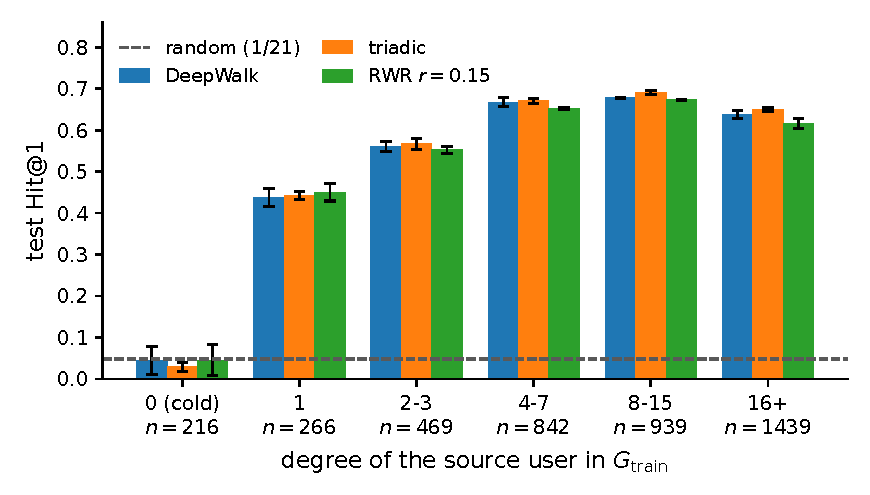
\includegraphics[width=0.82\textwidth]{fig_p1_degree.pdf}
\caption{Test Hit@1 by source degree for the baseline (DeepWalk), the best strategy
(triadic) and the worst (RWR); error bars are $\pm 1$ sd over seeds $\{0,1,2\}$.  The
cold-start bucket sits at chance for every strategy.}
\label{p1:fig:degree}
\end{figure}

\paragraph{Control.}
To check that the evaluation path itself carries no signal, I ran the identical pipeline
on a random Gaussian $Z$: it gives test Hit@1 $0.0671$ and MRR $0.2009$ (chance is
$1/21=0.0476$ and $0.1736$) and country test micro-F1 $0.1340$, far below the
majority-class rate of $0.2062$.  The learned embeddings are therefore genuinely doing
the work.

\subsection{Analysis}
\label{p1:sec:analysis}

\paragraph{The same embedding wins both tasks.}
The triadic walk is best in \emph{every} column of Table~\ref{p1:tab:comparison}, and
Figure~\ref{p1:fig:tradeoff} shows it alone in the top-right corner: there is no
homophily-versus-structural-equivalence trade-off to negotiate on this dataset.  That is
not an accident of the metrics --- both downstream tasks on this graph are homophily
tasks.  Friends of a user are found inside their community, and country is an extremely
assortative label on a social network (people mostly follow people in their own country),
so an embedding that sharpens community boundaries helps the link predictor and the
country classifier for the same reason.  A dataset where node labels were a function of
\emph{role} rather than community (bridges, hubs, peripherals) is where one would expect
the two tasks to pull apart, and where a $q>1$ walk should have paid off.

\paragraph{Which differences are real.}
Most of them are small, so the noise floor matters --- and it has to be read off the
\emph{test} columns.  \texttt{LinkPredictor.fit} selects $C$ on validation MRR and
\texttt{CountryClassifier.fit} selects $C$ on validation accuracy, so val H@1, val MRR and
val micro-F1 are measured on the very split that chose the model and their large ratios
($7.0\times$, $6.0\times$, $1.3\times$) are optimistic.  I therefore rest the argument on
the held-out columns: the between-strategy spread is $4.1\times$ the within-strategy sd
for test Hit@1, $4.2\times$ for test MRR and $3.9\times$ for test macro-F1.  Those are
real effects on data no model-selection decision ever saw.

But for country \emph{micro}-F1 the test spread is only $1.7\times$ the noise
($0.7607$--$0.7661$): \textbf{on micro-F1 the seven strategies are statistically
indistinguishable.}  Anyone reading only the micro-F1 column would conclude that the
sampling strategy does not matter; the macro-F1 columns show that it does, and by a wide
margin.  Test macro-F1 spreads $0.0240$ ($3.9\times$), and validation macro-F1 spreads
$0.0411$ --- $5.4\times$ its noise floor, the second-largest effect anywhere in this study,
with triadic at $0.6833$ against deg-corrected's $0.6421$.  Validation macro-F1 deserves a
little more trust than the other val columns, because $C$ is selected on validation
\emph{accuracy}, not macro-F1 --- macro-F1 is not the selection objective, merely measured
on the selection split --- and the unbiased test macro-F1 column agrees with it on both the
winner and the ordering.

This is exactly the imbalance effect the question points at: the label distribution runs
from $1{,}572$ users in the largest country to $16$ in the smallest (only $2$ of which land
in the $763$-user training split), so micro-F1 is dominated by a handful of big classes
that every embedding already gets right, and only macro-F1 is sensitive to what happens in
the tail.  Choosing a sampling strategy on micro-F1 would be choosing on noise.

\paragraph{node2vec buys nothing here.}
All three $(p,q)$ settings sit within noise of plain DeepWalk (test MRR $0.7184$,
$0.7196$, $0.7228$ versus $0.7207$), and the homophily-leaning setting $q{=}0.5$ is if
anything the \emph{worst} of the three.  I read this as a property of the graph rather
than of node2vec: with mean degree $5.1$ and $734$ components, a length-$40$ uniform walk
is already confined to a small neighbourhood, so re-weighting second-order transitions
has little room to change which nodes co-occur.  The second-order machinery costs a
doubling of sampling time and returns nothing measurable.

\paragraph{Why triadic works and the other two ideas do not.}
The triadic rule, $P(x)\propto 1+|N(v)\cap N(x)|$, prefers steps that close a triangle.
It is the only one of my three ideas that adds \emph{new information} --- it looks at the
graph two hops out, whereas uniform, RWR and degree-corrected walks only ever consult the
current node's neighbour list.  That extra information is precisely a community signal,
which is why its largest gains are on country macro-F1: $+0.0194$ on validation ($0.6833$
vs $0.6639$, $2.5$ noise-sds) and $+0.0141$ on test ($0.6974$ vs $0.6833$, $2.3$
noise-sds).  Macro-F1 is the metric that rewards getting the \emph{small} countries right,
and a small country is exactly the kind of tight, triangle-dense community that a
triangle-closing walk resolves best.
\begin{itemize}[label=$\bullet$,itemsep=1pt]
\item \textbf{RWR was my worst idea} (test MRR $0.7124$, $-0.0083$ against DeepWalk).  The
hypothesis --- that a personalised context sharpens pairwise proximity --- is falsified.
With a fixed length-$40$ budget, teleporting home $15\%$ of the time spends about six
tokens per walk re-emitting \texttt{start} and truncates the walk's effective reach, so
the corpus contains fewer distinct co-occurrences for the same cost.  The breakdown
localises the damage precisely: degree $1$ is the \emph{only} bucket where RWR beats
DeepWalk ($0.4499$ vs $0.4386$ test Hit@1, the largest degree-$1$ gain of any strategy ---
a short leash is exactly right when the source has one friend), and it is worse at every
degree $\ge 2$, by $-0.0218$ in the $\ge 16$ bucket.
\item \textbf{Degree-corrected sampling also failed} (test MRR $0.7121$, $-0.0086$) --- and
failed in an informative way.  The hypothesis was that suppressing hubs would lift the
\emph{low}-degree buckets; the measurement says the opposite happened.  It helped the
high-degree end ($+0.0099$ at $8$--$15$, $+0.0019$ at $\ge 16$) and did its worst damage
at $2$--$3$ ($-0.0199$).  Hubs are not noise to be corrected away: on a social graph a
shared popular contact is real evidence that two users belong together, and re-weighting
by $\deg(x)^{-1}$ discards exactly that evidence --- which hurts most for the sparse users
who had little other evidence to begin with.
\end{itemize}

\paragraph{Cold start is the real bottleneck, and no walk strategy can touch it.}
The single largest effect in this study is not a strategy at all.  Test Hit@1 runs from
$0.03$--$0.04$ at source degree $0$ to $0.68$--$0.69$ at degree $8$--$15$ --- a gap of
about $0.64$, roughly \emph{thirty-two} times the $0.0198$ that separates the best
strategy from the worst on that same metric.
The $666$ isolated users have no incident edge in $G_{\mathrm{train}}$, so
\texttt{sample\_walks} correctly returns \texttt{[]} for them and their embedding row is
zero \emph{by construction}.  The $216$ test queries with such a source are therefore
being scored from destination-side features alone, and the numbers confirm it exactly:
the cold bucket's seed-averaged Hit@1/MRR ($0.0447/0.1887$ for DeepWalk) match the
random-$Z$ control ($0.0671/0.2009$) and chance ($0.0476/0.1736$) rather than any learned
result.  Across all $21$ runs that bucket wanders between $0.0139$ and $0.1065$ with no
strategy stable across its own three seeds --- DeepWalk alone scores $0.0833$, $0.0231$,
$0.0278$.  What little ordering survives comes from a candidate-side popularity prior
rather than from anything the source's embedding contributes; Task~4 measures this
directly and finds none of the $216$ queries fully tied (median $20$ distinct scores of
$21$), so the run-to-run scatter is genuine instability, not tie-breaking.  Either way,
reading the cold-start column as evidence about a sampling strategy would be a mistake.  Fixing it
requires information from outside the observed social graph --- structural or profile
features, or the user--artist edges used in Task 4 --- not a better walk.

\paragraph{The non-monotone top bucket.}
Hit@1 peaks at degree $8$--$15$ and falls back for $\ge 16$ (seed-averaged
$0.6904 \to 0.6502$ for triadic).  More friends means more embedding evidence but also a
harder ranking problem: a high-degree user is plausibly connected to many of the $20$
sampled negatives, so the single held-out positive is genuinely harder to place first.
MRR falls much less than Hit@1 ($0.7959\to0.7744$), consistent with the positive still
being ranked near the top rather than lost.  These two top buckets are also where triadic
beats DeepWalk by the widest margin ($+0.0121$ and $+0.0125$ Hit@1, against $+0.0038$ at
degree $1$), which fits the same story: for a hub user, knowing \emph{which} community a
candidate belongs to is what separates the true friend from a plausible negative.

\paragraph{Practical conclusion.}
If I had to ship one embedding for both products, it would be the triadic walk: it is the
best on both tasks, it stays first-order, and it needs no $(p,q)$ tuning.  It is not free
--- sampling the whole $69{,}580$-walk corpus takes $1.9$\,s against DeepWalk's $0.7$\,s,
because each step draws from a precomputed weighted table rather than a plain list --- but
$1.9$\,s is negligible next to the $\approx 40$\,s of Skip-Gram training that follows it,
so the choice costs nothing that matters in practice.  But the honest headline is that
on this graph the choice of random-walk strategy moves test MRR by at most $1.3$ points,
while the degree of the query user moves it by about $60$ (from $0.19$ in the cold bucket
to $0.80$ at degree $8$--$15$); effort is better spent on the cold-start population than
on the sampler.
